\documentclass[11pt, A4paper,norsk]{article}
\usepackage[utf8]{inputenc}
\usepackage[T1]{fontenc}
\usepackage{babel}
\usepackage{amsmath}
\usepackage{amsfonts}
\usepackage{amsthm}
\usepackage[colorlinks]{hyperref}
\usepackage{listings}
\usepackage{color}
\usepackage{hyperref}
\usepackage{graphicx}
\usepackage{cite}

\definecolor{dkgreen}{rgb}{0,0.6,0}
\definecolor{gray}{rgb}{0.5,0.5,0.5}
\definecolor{daynineyellow}{rgb}{1.0,0.655,0.102}
\definecolor{url}{rgb}{0.1,0.1,0.4}

\lstset{frame=tb,
	language=Python,
	aboveskip=3mm,
	belowskip=3mm,
	showstringspaces=false,
	columns=flexible,
	basicstyle={\small\ttfamily},
	numbers=none,
	numberstyle=\tiny\color{gray},
	keywordstyle=\color{blue},
	commentstyle=\color{daynineyellow},
	stringstyle=\color{dkgreen},
	breaklines=true,
	breakatwhitespace=true,
	tabsize=3
}

\lstset{inputpath="C:/Users/Torstein/Documents/UiO/Mat1110/Python programmer"}
\hypersetup{colorlinks, urlcolor=url}

\author{Torstein Solheim Ølberg}
\title{Svar på Oblig nr.1 i Mat1110}

\begin{document}
\maketitle
	\begin{center}
\Large \textbf{Oppgaver}
	\end{center}
		\paragraph{1a)}
			\begin{flushleft}
La $T$ være en lineæravbildning $T : \Re^2 \rightarrow \Re^2$ som er slik at 
$$T
\left(\begin{tabular}{ c }
2 \\
1
\end{tabular} \right)
=
\left(\begin{tabular}{ c }
-2 \\
1
\end{tabular} \right)
\text{ og }
T
\left(\begin{tabular}{ c }
1 \\
1
\end{tabular} \right)
=
\left(\begin{tabular}{ c }
1 \\
1
\end{tabular} \right)$$ \\
Finn en $2 \times 2$ matrise $A$ slik at $A\vec{x} = T\vec{x}$ for alle $\vec{x} \in \Re^2$ \\
\vspace{1mm}
\textbf{Løsning:} \\
				\begin{align}
T = 
\left( \begin{tabular}{ c c }
t_{11} & t_{12} \\
t_{21} & t_{22}
\end{tabular} \right) \\
\text{det betyr at A er på samme form} \nonumber \\
A = 
\left(\begin{tabular}{ c c }
a_{11} & a_{12} \\
a_{21} & a_{22}
\end{tabular} \right) 
\hspace{10mm} 
\vec{x} = 
\left(\begin{tabular}{ c }
2 \\
1
\end{tabular} \right) \\
2 \cdot a_{11} + a_{12} = -2 \\
2 \cdot a_{21} + a_{22} = 1 \\
a_{11} + a_{12} = 1 \\
a_{21} + a_{22} = 1 \\
a_{11} = \frac{-2 - a_{12}}{2} \hspace{10mm} a_{11} = 1 - a_{12} \\
\text{Setter den ene ligningen lik den andre} \nonumber \\
1 - a_{12} = \frac{-2 - a_{12}}{2} \Rightarrow \frac{a_{12}}{2} = 2 \Rightarrow a_{12} = 4 \\
\text{Da kan jeg regne ut $a_{11}$ ved å sette inn verdi for $a_{12}$} \nonumber \\
a_{11}  = 1 - 4 \Rightarrow a_{11} = -3 \\
\text{gjør det samme for de to andre ligningene} \nonumber \\
a_{21} = \frac{1 - a_{22}}{2} \hspace{10mm} a_{21} = 1 - a_{22} \\
1 - a_{22} = \frac{1 - a_{22}}{2} \Rightarrow \frac{1}{2}a_{22} = \frac{1}{2} \Rightarrow a_{22} = 1 \\
a_{21} = 1 - 1 \Rightarrow a_{21} = 0 \\
A = 
\left(\begin{tabular}{ c c }
-3 & 4 \\
0 & 1
\end{tabular} \right)
				\end{align}
			\end{flushleft}
		\paragraph{b)}
			\begin{flushleft}
Finn to egenverdier og to tilhørende egenvektorer for $A$. \\
\vspace{1mm}
\textbf{Løsning:} \\
\vspace{1mm}
				\begin{align}
A\vec{x} = \lambda\vec{x} \\
\text{da må:} \nonumber \\
-3x_1 + 4x_2 = \lambda x_1 \\
0 \cdot x_1 + x_2 = \lambda x_2 \Rightarrow x_2 = \lambda x_2 \\
\text{Dette fungerer hvis $\lambda = 1$ og $x_1 = x_2$ eller $x_2 = 0$ og $\lambda = -3$}
				\end{align}
Dette betyr at en egenverdi er $\lambda = 1$ og at en tilhørende egenvektor kan være $\vec{x} = 
\left(\begin{tabular}{ c }
2 \\
2
\end{tabular} \right)$. En annen egenverdi kan være $\lambda = 0$ og at tilhørende egenvektor kan være $\vec{x} = 
\left(\begin{tabular}{ c }
2 \\
0
\end{tabular} \right)$.
			\end{flushleft}
		\paragraph{c)}
			\begin{flushleft}
Regn ut $$(A^5 + A^3 + A)
\left(\begin{tabular}{ c }
2 \\
1
\end{tabular} \right) $$ \\
\vspace{1mm}
\textbf{Løsning:} \\
\vspace{1mm}
				\begin{align}
A^3 = 
\left(\begin{tabular}{ c c }
-3 & 4 \\ 
0 & 1 
\end{tabular} \right)
\left(\begin{tabular}{ c c }
-3 & 4 \\ 
0 & 1 
\end{tabular} \right)
\left(\begin{tabular}{ c c }
-3 & 4 \\ 
0 & 1 
\end{tabular} \right)
=
\left(\begin{tabular}{ c c }
-27 & 28 \\ 
0 & 1 
\end{tabular} \right) \nonumber \\
A^5 = 
\left(\begin{tabular}{ c c }
-27 & 28 \\ 
0 & 1 
\end{tabular} \right)
\left(\begin{tabular}{ c c }
-3 & 4 \\ 
0 & 1 
\end{tabular} \right)
\left(\begin{tabular}{ c c }
-3 & 4 \\ 
0 & 1 
\end{tabular} \right) 
=
\left(\begin{tabular}{ c c }
-243 & 244 \\ 
0 & 1 
\end{tabular} \right) \nonumber \\
(A^5 + A^3 + A) = 
\left(\begin{tabular}{ c c }
-243 -27 -3 & 244 + 28 + 4 \\ 
0 + 0 + 0 & 1 + 1 + 1 
\end{tabular} \right)
=
\left(\begin{tabular}{ c c }
-273 & 276 \\
0 & 3
\end{tabular} \right) \nonumber \\
\left(\begin{tabular}{ c c }
-273 & 276 \\ 
0 & 3
\end{tabular} \right)
\left(\begin{tabular}{ c }
2 \\
1 
\end{tabular} \right)
=
\left(\begin{tabular}{ c }
-270 \\
3
\end{tabular} \right) \nonumber
				\end{align}
			\end{flushleft}
		\paragraph{2a)}
			\begin{flushleft}
En disk med radius $\rho \leq \frac{1}{2}$ ruller på parabelen $y = x^2$. Se figur 1. La senteret i disken ha koordinater $(X, Y)$. \\
Finn enhetsnormalen med negativ andrekomponent til kurven $s(x) = (x, x^2)$. Nedenfor kaller
vi denne for $\vec{n}(x)$. \\
\vspace{1mm}
\textbf{Løsning:} \\
\vspace{1mm}
Vi finner enhetstangenten til $s(x)$ ved å derivere denne vektoren og dele på lengden av vektoren.
$$\frac{s'(x)}{|s'(x)|} = \frac{(1, 2x)}{|(1, 2x)|} = \frac{(1, 2x)}{\sqrt{1 + 4x^2}}$$
Hvis vi da krysser denne vektoren med $\vec{k}$ så får vi enhetsnormalen til punktet. \\
\left| \begin{tabular}{ c c c }
$\vec{i}$ & $\vec{j}$ & $\vec{k}$ \\
$\dfrac{1}{\sqrt{1 + 4x^2}}$ & $\dfrac{-2x}{\sqrt{1 + 4x^2}}$ & 0 \\
0 & 0 & 1
\end{tabular} \right|
$$\Rightarrow \vec{n} = \left(\frac{2x}{\sqrt{1 + 4x^2}}, - \frac{1}{\sqrt{1 + 4x^2}}\right)$$ \\

			\end{flushleft}
		\paragraph{b)}
			\begin{flushleft}
Finn $X$ og $Y$ som funksjon av førstekomponten til berøringspunktet $s(x)$ \\
\vspace{1mm}
\textbf{Løsning:} \\
\vspace{1mm}
				\begin{align}
(X, Y) = s(x) - \rho n(x) \\
(X, Y) = (x, x^2) - rho (\frac{2x}{\sqrt{1 + 4x^2}}, - \frac{1}{\sqrt{1 + 4x^2}}) \\
(X, Y) = (x - \frac{2\rho x}{\sqrt{1 + 4x^2}}, x^2 + \frac{\rho}{\sqrt{1 + 4x^2}}) 
				\end{align}
			\end{flushleft}
		\paragraph{c)}
			\begin{flushleft}
Anta at $x(t) = 2 cos(t)$. Finn hastigheten $\vec{v}(t)$ og akselerasjonen $a(t)$ til senteret i disken. \\
\vspace{1mm}
\clearpage
\textbf{Løsning:} \\
\vspace{1mm}
				\begin{align}
(X, Y)' = \left(2cos(t) - \frac{2 \cdot 2 \rho cos(t)}{\sqrt{1 + 4 \cdot 2^2 cos^2(t)}}, 4cos^2(t) + \frac{\rho}{\sqrt{1 + 4 \cdot 2^2 cos^2(t)}}\right)' \nonumber \\
v_x = \left(2cos(t) - \frac{4 \rho cos(t)}{\sqrt{1 + 16cos^2(t)}}\right)' \nonumber\\
v_x = -2sin(t) -  \frac{4 \rho sin(t)}{\sqrt{1 + 16cos^2(t)}} + \frac{64 \rho sin(t)cos^2(t)}{\sqrt{1 + 16cos^2(t)}^3}\nonumber \\
v_y = \left(4cos^2(t) + \frac{\rho}{\sqrt{1 + 16cos^2(t)}}\right)' \nonumber \\
v_y = -8cos(t)sin(t) - \frac{16 \rho sin(t)cos(t)}{\sqrt{1 + 16cos^2(t)}} \nonumber \\
v(x) = \left(-2sin(t) -  \frac{4 \rho sin(t)}{\sqrt{1 + 16cos^2(t)}} + \frac{64 \rho sin(t)cos^2(t)}{\sqrt{1 + 16cos^2(t)}^3}, -8cos(t)sin(t) - \frac{16 \rho sin(t)cos(t)}{\sqrt{1 + 16cos^2(t)}}\right) \nonumber \\
a_x = v_x' \nonumber \\
a_x = -2cos(t) - \frac{4 \rho cos(t)}{\sqrt{1 + 16cos^2(t)}} \nonumber \\
- \frac{64 \rho sin^2(t)cos(t)}{\sqrt{1 + 16cos^2(t)}^3} \nonumber \\
+ \frac{64 \rho cos^3(t) \nonumber - 128sin^2(t)cos(t)}{\sqrt{1 + 16cos^2(t)}^3} \nonumber \\
+ \frac{3072 \rho sin^2(t)cos^3(t)}{\sqrt{1 + 16cos^2(t)}^5} \nonumber \\
a_y = v_y' \nonumber \\
a_y = -8cos^2(t) + 8sin^2(t) \nonumber \\
- \frac{16 \rho (cos^2(t) - sin^2(t))}{\sqrt{1 + 16cos^2(t)}} \nonumber \\
+ \frac{64 \rho sin(t)cos^2(t)}{\sqrt{1 + 16cos^2(t)}^3} \nonumber
				\end{align}
\vspace{1mm}
			\end{flushleft}
		\paragraph{d)}
			\begin{flushleft}
Vi er nå interessert i å finne banen, $\vec{r}(x)$, til det punktet på randen av disken som er slik at $\vec{r}(0) = (0, 0)$. For å hjelpe oss med dette innfører vi funksjonen
$$\sigma(x) = \int_{0}^{x} \sqrt{1 + 4\xi^2} d\xi = \frac{1}{4} \left(2x\sqrt{1 + 4x^2} + sinh^{-1}(2x) \right)$$ \nonumber
der $sinh^{-1}$ betegner den inverse til $hyperbolsk sinus$. \\
Forklar hvorfor $\sigma(x)$ er buelengden på kurven $\vec{s}(t) = (t, t^2)$ for $t \in [0, x]$.
\vspace{1mm}
\textbf{Løsning:} \\
\vspace{1mm}
Buelengden til $f(\vec{x})$ fra $a$ til $b$ er $\int_{0}^{x} |\vec{x}'|$ \\
$s(t) = (t, t^2) \hspace{5mm} s' = (1, 2t)$ \\
Buelengden til $s = \int_{0}^{x} \sqrt{1^2 + (2t)^2}dt = \int_{0}^{x} \sqrt{1 + 4t^2}$
			\end{flushleft}
		\paragraph{e)}
			\begin{flushleft}
La $m(x) = \vec{r}(x) - (X(x), Y(x))$. Forklar hvorfor \\
$\vec{m}(x) = \rho$
\left( \begin{tabular}{ c c }
$cos(\frac{\sigma(x)}{\rho})$ & $sin(\frac{\sigma(x)}{\rho})$ \\
$-sin(\frac{\sigma(x)}{\rho})$ & $cos(\frac{\sigma(x)}{\rho})$
\end{tabular} \right) $n(x)$ \\
\vspace{1mm}
\textbf{Løsning:} \\
\vspace{1mm}
Banen til punktet på randen av disken som er slik at $\vec{r}(0) = (0, 0)$ minus banen til banen til sentrum av disken er en vektor som roterer rundt i ring med lengde $\rho$ og samme retning $\vec{n}(x)$. Matrisen vi ser i oppgaven over er en rotasjonsmatrise som roterer linja rundt i ring og vinkelen finner vi ved å ta buelengden og dele på radien i sirkelen.
			\end{flushleft}
		\paragraph{f)}
			\begin{flushleft}
Anta at $\rho = 1/2$, bruk Matlab eller python til å plotte kurvene $s(x)$, $X(x), Y(x)$ og $r(x)$ for $x \in [−2, 2]$ i samme diagram. \\
\vspace{1mm}
\textbf{Løsning:} \\
\vspace{1mm}
				\begin{align}
\vec{s}(x) = (x, x^2) \nonumber \\
(\vec{X}(x), \vec{Y}(x)) = s(x) - \rho*\vec{n}(x) \nonumber \\
\vec{r}(x) = \vec{m}(x) + (\vec{X}(x), \vec{Y}(x)) \nonumber
				\end{align}
\lstinputlisting{Oblig1_2f.py}
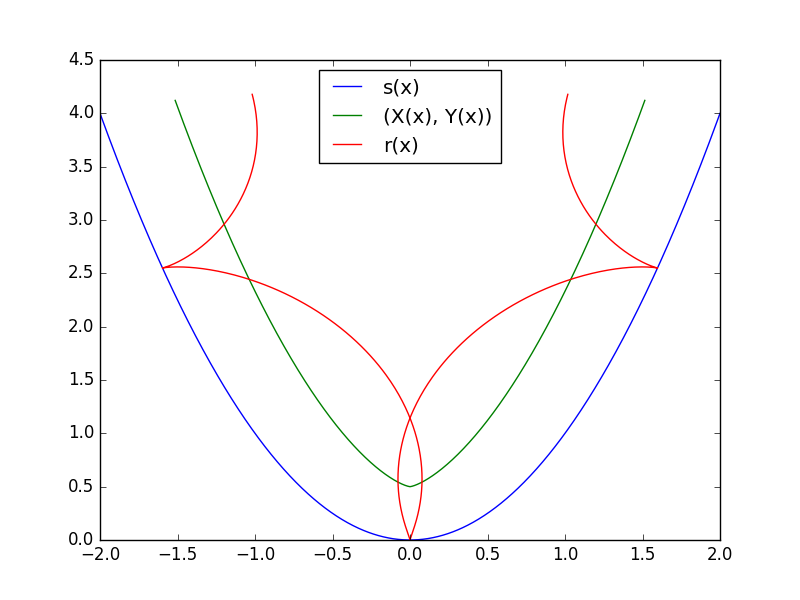
\includegraphics[width=12.6cm,height=8cm]{C:/Users/Torstein/Documents/UiO/Mat1110/Python programmer"/Oblig1_2f.png}
				\end{flushleft}
		\paragraph{3a)}
			\begin{flushleft}
La $\sigma(t)$ være kurven $\sigma(t) = cos(t)\vec{i} + sin(t)\vec{j}$, og sett $r(t) = e^{- t}\sigma(t)$. \\
Skissér kurven $r(t)$ for $t \in [0, 4\pi]$. \\
\vspace{1mm}
\textbf{Løsning:} \\
\vspace{1mm}
\lstinputlisting{Oblig1_3a.py}
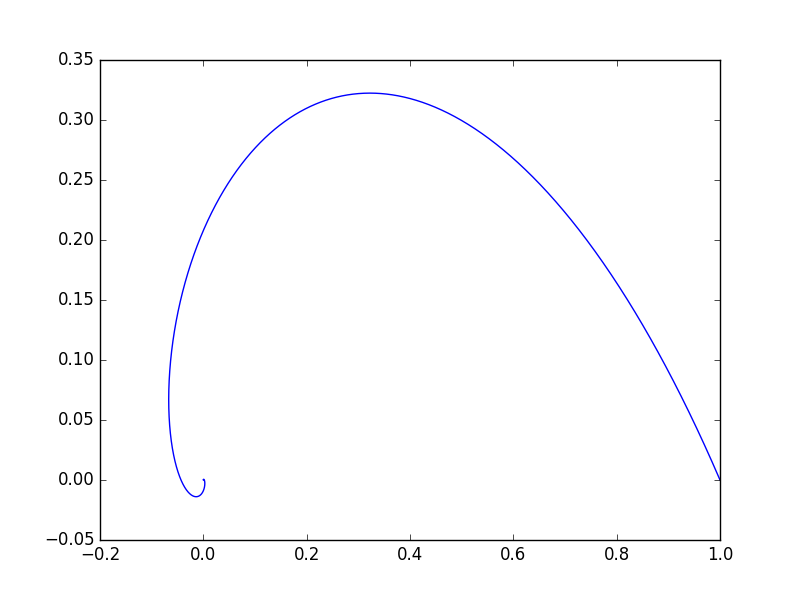
\includegraphics[width=12.6cm,height=8cm]{C:/Users/Torstein/Documents/UiO/Mat1110/Python programmer"/Oblig1_3a.png}
			\end{flushleft}
		\paragraph{b)}
			\begin{flushleft}
Finn lengden av linjestykket $r(t)$ for $t \in [0, \infty)$.
\vspace{1mm}
\textbf{Løsning:} \\
\vspace{1mm}
				\begin{align}
L(\vec{r}) = \int_{0}^{\infty} \sqrt{(e^{- t}cos(t))'^2 + (e^{- t}sin(t))'^2} dt \nonumber\\
L(\vec{r}) = \lim_{a \rightarrow \infty} \int_{0}^{a} \sqrt{(-e^{- t}cos(t) - e^{-t}sin(t))^2 + (-e^{- t}sin(t) + e^{-t}cos(t))^2} dt \nonumber \\
L(\vec{r}) = \lim_{a \rightarrow \infty} \sqrt{2} \int_{0}^{a} \sqrt{e^{-2t}sin^2(t) + e^{- 2t}cos^2(t)} dt \nonumber \\
L(\vec{r}) = \lim_{a \rightarrow \infty} \sqrt{2} \int_{0}^{a} \sqrt{e^{-2t}} dt \nonumber \\
L(\vec{r}) = \lim_{a \rightarrow \infty} \sqrt{2} \left[ -e^{-t} \right]_{0}^{a} = \lim_{a \rightarrow \infty} \sqrt{2}(-e^{-a} + e^{-0}) = \sqrt{2}(0 + 1) = \sqrt{2} \nonumber
				\end{align}
			\end{flushleft}
		\paragraph{c)}
			\begin{flushleft}
Vis at $r(t)$ tilfredsstiller differensialligningen \\
$$ \vec{r}'(t) =
- \left( \begin{tabular}{ c c }
1 & 1 \\
-1 & 1
\end{tabular} \right) \vec{r}(t), \hspace{5mm} \vec{r}(0) = \vec{i}$$ \\
\vspace{1mm}
\textbf{Løsning:} \\
\vspace{1mm}
				\begin{align}
\vec{r}(t) = e^{-t}(cos(t)\vec{i} + sin(t)\vec{j}) \nonumber\\
\vec{r}'(t) = (-e^{-t}cos(t) - e^{-t}sin(t))\vec{i} + (-e^{-t}sin(t) + e^{-t}cos(t))\vec{j} \nonumber \\
\vec{r}'(t) =
- \left( \begin{tabular}{ c c }
1 & 1 \\
-1 & 1
\end{tabular} \right) e^{t}(cos(t)\vec{i} + sin(t)\vec{j}) \nonumber \\
\vec{r}'(t) = -(e^{-t}cos(t) - e^{-t}sin(t))\vec{i} - (-e^{-t}cos(t) + e^{-t}sin(t))\vec{j} \nonumber \\
\vec{r}'(t) = -(e^{-t}cos(t) - e^{-t}sin(t))\vec{i} + (-e^{-t}sin(t) + e^{-t}cos(t))\vec{j} \nonumber
				\end{align}
			\end{flushleft}
		\paragraph{4a)}
			\begin{flushleft}
Vi lar $x = (x_1, \dots, x_n)$ betegne en vektor i $\Re^n$. Et vektorfelt $F : \Re^n \rightarrow \Re^n$ kalles $sentralt$ hvis det kan skrives på formen $F(x) = f(|x|)x$, der $f$ er en funksjon fra $[0, \infty) \rightarrow \Re$. \\
Vis at sentrale vektorfelter konservative i $\Re^n$ hvis $f$ er kontinuerlig deriverbar og $\lim_{r \rightarrow 0} f'(r) = 0$. \\
\vspace{1mm}
\textbf{Løsning:} \\
\vspace{1mm}
Vi ser av teorem 3.5.3 sier at hvis det finnes en funksjon $\phi(\vec{x})$ som tilfredstiller at $\nabla \phi(\vec{x})$ for alle $\vec{x} \in A$ så er $F$ konservativ. hvis vi da kan finne en funksjon som har graduent lik $F$ så har vi bevist at dette er et konservativt felt fordi den er kontinuerlig deriverbar og deriverbar i punktet $0$.
				\begin{align}
\text{Vi velger} \phi (\vec{x}) = - \frac{k}{|\vec{x}|} \nonumber \\
\phi (\vec{x}) = -k(x_1^2 + \cdots + x_n^2)^{-\frac{1}{2}} \nonumber \\
\frac{\partial \phi}{\partial x_i} = -k(- \frac{1}{2})(x_1^2 + \cdots + x_n^2)^{- \frac{3}{2}}2x_i = \frac{k}{|\vec{x}|^3}\vec{x}_i \nonumber \\
\nabla \phi (\vec{x}) = \frac{k}{|\vec{x}|^3}(x_1, \dots , x_n) = \frac{k}{|\vec{x}|^3}\vec{x} \nonumber
				\end{align}
Nå gjenstår det bare å sette $f(|\vec{x}|) = \frac{k}{|\vec{x}|^3}$ og da blir jo $F(\vec{x}) = \nabla \phi(\vec{x})$, altså har vi bevist at $F$ er et konservativt felt.
			\end{flushleft}
		\paragraph{4b)}
		\begin{flushleft}
La $h(r)$ være en funksjon slik at $h'(r) = rf(r)$. Vis at $\phi(\vec{x}) = h(|\vec{x}|)$ er en potensialfunksjon til $F$. \\
\vspace{1mm}
\textbf{Løsning:} \\
\vspace{1mm}
Hvis $h'(r) = rf(r)$ og $\phi(\vec{x}) = h(|\vec{x}|)$ det betyr at
$\phi(\vec{x}) = \vec{x}f(|\vec{x}|)$ som vi allerede viste i forrige oppgave.
		\end{flushleft}
\end{document}